\section{Experimental Design and Evaluation Protocol}
\label{sec:design}

This section separates what has been done from what is planned. Three things have been done: the benchmark was downloaded, verified and sampled; a 50-case seed set was frozen; and an operational smoke capture of OpenAlex responses was captured and replayed offline. Everything else is planned: the independent label audit, the affiliation-cleaning decision, the main sample, the main evaluation and the statistical analysis. Fig.~\ref{fig:pipeline} shows the workflow, and the planned stages are drawn with dashed outlines.

\begin{figure*}[t]
\centering
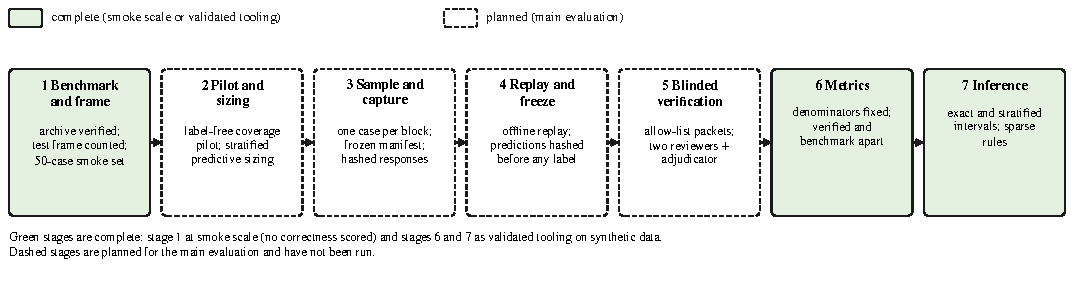
\includegraphics[width=\textwidth]{figures/evaluation_pipeline.pdf}
\caption{Experimental workflow. Completed stages ran at smoke scale only. The label audit, the evaluation and the analysis are planned. Regenerate with \texttt{figures/make\_figures.py}.}
\label{fig:pipeline}
\end{figure*}

\subsection{Benchmark}
\label{sec:benchmark}
The primary benchmark candidate is LAGOS-AND, version 2.0, released on Zenodo (DOI 10.5281/zenodo.7313353) under a CC~BY~4.0 licence~\cite{zhang2022lagosandv2}. The dataset paper describes its construction from ORCID and DOI evidence~\cite{zhang2023lagosand}.
% TODO: confirm from the dataset paper and the Zenodo record how the ORCID attribution of each publication record was established, and whether the v2.0 release changed it.
We used the block-trimmed archive. Its size (743,558,936 bytes) and MD5 checksum matched the values listed by Zenodo, the compressed stream was read to its end, and we computed and recorded a SHA-256 checksum. The archive was processed by streaming and deleted afterwards. Table~\ref{tab:dataset} gives the characteristics we measured.

\begin{table}[t]
\caption{LAGOS-AND v2.0 (block-trimmed) as measured by the preparation script.}
\label{tab:dataset}
\centering
\footnotesize
\renewcommand{\arraystretch}{1.1}
\begin{tabular}{@{}p{0.55\columnwidth}p{0.33\columnwidth}@{}}
\toprule
\textbf{Characteristic} & \textbf{Value} \\
\midrule
Data rows & 1,476,550 \\
Name blocks & 80,294 \\
(block, ORCID) identity groups & 244,564 \\
ORCIDs occurring in more than one block & 0 \\
DOIs shared by more than one ORCID & 0 \\
Publication years & 1870 to 2022 \\
Rows without an author affiliation & 14.10\% \\
Blocks eligible for sampling & 70,351 \\
\bottomrule
\end{tabular}
\end{table}

Each block collects publication records for one printed name form, and each identity group within it is defined by an ORCID value attached to its records. Fourteen columns are present, including the printed author name, affiliation, DOI, publication year, coauthor names and a train, test or validation flag. The \texttt{pid} column behaves like a Microsoft Academic Graph identifier and is not an OpenAlex identifier, and we do not treat it as one. Coauthors are given as name strings without identifiers, so the coauthor-ID signal cannot be observed on this dataset.

The ORCID basis of the groups creates a circularity risk. The expected identity is defined by ORCID equality, and OpenAlex candidate profiles also carry an ORCID field; the two may derive from overlapping upstream attributions. Agreement on ORCID may then reflect shared attribution and not independent verification of the person, and an error in an ORCID attribution could be present on both sides. \textbf{ORCID equality is therefore a provisional matching mechanism and not independent identity ground truth.} The ORCID field also bounds what it can label: in the smoke capture it held a value for only 57.5\% of returned candidates. These are the reasons for the independent audit of Section~\ref{sec:audit}.

\subsection{Seed Preparation}
\label{sec:seeds}
A deterministic sampler (seed 20261119) built the 50-case smoke sample. The unit of sampling is a complete name block. Blocks with more than eight ORCID groups (2,391) and blocks in which no group has two distinct DOIs (7,552) were excluded. Eligible blocks were stratified by block size alone, using the number of unique DOIs (0--9, 10--49, 50--199 and 200 or more), ordered within each stratum by a hash of the seed and the block name, and taken round-robin only if every query-eligible group of a block fitted the target. No OpenAlex result, ORCID match or HAMMER output was used. The sample has 50 cases from 23 blocks (6, 6, 6 and 5 blocks in the four strata), with 32 train, 15 test and 3 validation cases according to the source flag. HAMMER does not train, so the flag records provenance only. Re-running the sampler on the archive reproduced every output byte for byte, apart from the recorded sampling date.

A seed contains an opaque case identifier, the printed name, an opaque group and block identifier, the context for C1 and for C1x, and sampling metadata. It contains no ORCID, no \texttt{pid} and no coauthor field. The primary C1 context is the affiliation of one designated citation of the group, normalized as described in Section~\ref{sec:affiliation}, and that citation's publication year as a one-year active range. The designated citation is the one with the smallest hash of the seed, ORCID and DOI among those that have an affiliation. Two cases have no affiliation, so their C1 context has no institution. The designated citation is a property of a group member, so it carries a weak hint of group membership. It is the kind of information a user would hold about a new paper, and we record the hint as a design limitation.

The DOI register holds 1,713 DOIs, each used by exactly one case: 1,663 registered as \texttt{gold\_evidence} (the group's other citations) and 50 as \texttt{both} (the designated citation, with a written justification). None is registered as \texttt{query\_context}, so no DOI is present in C1. The 50 designated DOIs form the C1x context. The seeds and the register were hashed and frozen before any candidate was generated.

These 50 cases are an operational pilot sample and are not the main evaluation sample. They are also not 50 independent observations, because the cases come from 23 blocks and cases within a block are related.

\subsection{Smoke Capture}
\label{sec:smoke}
The smoke capture checked whether the toolkit and the provider interface work end to end. It scored no correctness. The capture issued 92 requests, all of which returned HTTP 200: 42 author searches and 50 DOI-based works look-ups for C1x. Fifty cases need 42 and not 50 author searches because R0 and R2 issued identical primary requests in every case and therefore shared one response, ten cases repeat another case's printed name and share its request, and two initials fallbacks were issued. Every response was written to its own file and hashed before the next request. All 92 hashes verified, and the offline replay reproduced its four artifacts byte for byte across two runs. The provider-reported cost was \$0.047. An earlier attempt used a placeholder credential and received 40 HTTP 401 responses. Its records are preserved separately and are not part of the data. The capture now stops at once on HTTP 401, 403 or 429, after saving and hashing the response.

\begin{table}[t]
\caption{Smoke-capture retrieval diagnostics (50 cases, 23 blocks). The expected ORCID is the dataset's, so these counts show label availability and not identity accuracy.}
\label{tab:smoke-retrieval}
\centering
\footnotesize
\renewcommand{\arraystretch}{1.1}
\begin{tabular}{@{}p{0.60\columnwidth}p{0.10\columnwidth}p{0.10\columnwidth}@{}}
\toprule
\textbf{Diagnostic (denominator 50)} & \textbf{R0} & \textbf{R2} \\
\midrule
Expected ORCID found in the pool & 36 & 38 \\
Expected-ORCID profile ranked first & 21 & 22 \\
Expected-ORCID profile within first 5 & 32 & 34 \\
Expected ORCID absent from a successful pool & 7 & 7 \\
ORCID null in every returned candidate & 5 & 5 \\
Successful empty pool & 2 & 0 \\
Provider failure or malformed response & 0 & 0 \\
\bottomrule
\end{tabular}
\end{table}

Table~\ref{tab:smoke-retrieval} lists the retrieval diagnostics. The ORCID field was present on every returned candidate, with a value for 57.5\% of them. The two R0 pools that were empty were found by R2's initials fallback, and the other 48 pools were identical. Rank is the provider's order. These counts describe an ORCID-based diagnostic on one small sample. They do not validate identity retrieval accuracy, and they cannot support a comparison of R0 and R2, because the two shared their primary response in all 50 cases.

\begin{table}[t]
\caption{Smoke-capture replay outcomes (50 cases). No correctness is scored.}
\label{tab:smoke-replay}
\centering
\footnotesize
\renewcommand{\arraystretch}{1.1}
\begin{tabular}{@{}p{0.50\columnwidth}p{0.11\columnwidth}p{0.11\columnwidth}@{}}
\toprule
\textbf{Configuration} & \textbf{Auto} & \textbf{Manual} \\
\midrule
C0, selective\_policy\_v2 & 0 & 50 \\
C1, selective\_policy\_v2 & 4 & 46 \\
C1x (exploratory), selective\_policy\_v2 & 7 & 43 \\
\bottomrule
\end{tabular}
\end{table}

Table~\ref{tab:smoke-replay} lists the replay outcomes under the full policy; every case was either automatic or manual, and none fell into the unresolved, empty-retrieval, provider-failure or no-score categories. The zero in C0 follows from the policy under name-only evidence (Section~\ref{sec:policy}) and is not evidence of safety. C1x remains exploratory: its publication evidence comes from a DOI that is a member of the group, and publication overlap was observed for the top candidate in all 50 cases. Under the threshold-gate ablation with P3 relaxation, C1x yields 26 automatic outcomes, so the safeguard blockers withhold automation in many of the cases that would otherwise pass the threshold gates; whether this improves precision has not been measured. In C1 the institution signal was observed for the top candidate in 29 cases, the candidate had no affiliation in 19 and the query had none in 2, and the temporal signal was observed in 36 and inconclusive in 14. Signal availability, and not only the score, therefore drives the outcome. These counts do not support any claim of precision, recall or superiority over a baseline.

\subsection{Independent Label Audit}
\label{sec:audit}
The independent label-validity audit has not been started. It is planned for about 30 cases and is a study of the validity of the automatic labels. It is not a substitute for independent labels in the main evaluation, and it does not validate the 50 smoke cases. For each audited case it must separate four questions: whether an OpenAlex profile represents the expected person; whether several OpenAlex profiles represent the same person; whether the expected person is absent from the returned pool; and whether the available evidence is insufficient to decide. Its aim is to estimate the error rate of the automatic ORCID-based labels.

Reviewers cannot see the expected ORCID, yet they still need enough information to identify the person and to compare candidate profiles. We therefore plan \emph{blinded candidate dossiers}. A dossier hides the expected ORCID, and it hides all HAMMER scores, ranks and decisions. It also hides the ORCID field of each candidate profile wherever that field could reveal the benchmark label. It retains independently verifiable evidence, such as publisher records, institutional profiles and publication authorship, and it presents each candidate under an opaque identifier. The mapping from opaque identifiers to provider identifiers is kept in a separate file that reviewers cannot access. Two reviewers work independently, and a third person adjudicates disagreements. Evidence from outside OpenAlex is used wherever it exists. Cases that cannot be verified independently remain \emph{uncertain} or \emph{unverified}. They are never forced into a label, they are excluded from the primary rates, and their number is reported.
% TODO: fix the dossier contents, the evidence sources, the review form and the comparison between the adjudicated mapping and the automatic ORCID mapping before the audit starts. The current plan comes from the feasibility report, not from a frozen protocol file.

Main-evaluation cases need defensible labels as well. How they will be obtained for a sample larger than the audit is not yet decided, and no main-evaluation claim will rest on unaudited ORCID equality alone.

\subsection{Affiliation Cleaning}
\label{sec:affiliation}
Affiliations in the benchmark contain source markers. The seed builder replaces the tab marker \texttt{\#TAB\#} with a space and collapses whitespace, and it keeps the original string in a separate file. Other markers, \texttt{\#R\#\#N\#} and \texttt{\#N\#}, were observed in the sample and are not handled, and some strings contain long multi-institution text. Extending the rule would change the frozen seed and would therefore define a new dataset version. Whether and how to extend it is undecided. The requirements are that the raw affiliation is always preserved, that every transformation is documented, and that the normalizer is separately versioned. No cleaning beyond the tab marker has been done.

\subsection{Main Evaluation and Statistical Plan}
\label{sec:main}
The main evaluation has not been run, and no result of it is reported. Its sample size, sampling frame and analysis details are not yet fixed, and we state none here. The sample size will not be decided until the audit process and the statistical design are settled.
% TODO: record the main sample size, the blocks or identity groups drawn, and the frozen configuration after the director's decision; do not invent a size.

The sample will consist of new cases and will not reuse the smoke cases for confirmatory claims. The thresholds, weights, policy version and code revision will be frozen and recorded before any candidate is captured for it, and no setting will be tuned on its results. Uncertain labels will be excluded from primary rates and counted.

The smoke sample has 50 cases from 23 blocks, and cases within a block are related, so they are clustered observations and not 50 independent ones. For the confirmatory sample we prefer one case per independent block, where that is feasible. If several cases per block are necessary, inference will be block-clustered. The number of blocks will be reported together with the number of cases. An interval will not be computed as though cases from the same block were independent.
% TODO: choose the block-clustered inference method (for example a cluster bootstrap) before unsealing; none is chosen yet.

\subsection{Evaluation Metrics}
\label{sec:metrics}
Table~\ref{tab:metrics} defines the planned measures and their denominators. Let $R$ be the audited cases with a resolved expected identity, $M\subseteq R$ those having at least one mapped profile in the captured pools, and $E$ the audited cases with a resolved or unresolved label (uncertain cases excluded and counted). A \emph{correct automatic assignment} is an automatic selection that is a mapped profile of the expected person of a resolved case. An automatic selection on an unresolved control, or on a case whose person has no profile in the pool, is a false automatic assignment.

Retrieval is reported in two complementary ways. \emph{Conditional} Recall@$k$ is computed among the cases in $M$, that is, among cases where a mapped profile exists in the captured pool, and asks how often it is ranked within the first $k$. \emph{End-to-end} retrieval success@$k$ is computed among all cases in $R$ and asks how often a mapped profile is present within the first $k$. The conditional measure alone would let a retriever look effective by excluding the cases in which it retrieved nothing, so the two are always shown together. The \emph{candidate-pool mapping rate} $|M|/|R|$ is the share of resolved cases whose expected person has a mapped profile in the captured pools. It does not measure the provider's catalog: a failed search does not show that the person is absent from OpenAlex, which would need a separate source-coverage investigation.

\begin{table*}[t]
\caption{Planned metrics and denominators. Every rate is reported with its numerator and denominator.}
\label{tab:metrics}
\centering
\footnotesize
\renewcommand{\arraystretch}{1.12}
\begin{tabular}{@{}p{0.19\textwidth}p{0.47\textwidth}p{0.26\textwidth}@{}}
\toprule
\textbf{Measure} & \textbf{Definition} & \textbf{Denominator} \\
\midrule
Candidate-pool mapping rate & Resolved cases with a mapped profile in the captured pools & $|R|$ \\
Conditional Recall@$k$, $k\in\{1,5,10\}$ & Cases whose first mapped profile is within the first $k$ provider-ordered candidates & $|M|$ \\
End-to-end success@$k$ & Cases with a mapped profile within the first $k$ provider-ordered candidates & $|R|$ \\
MRR, conditional and end-to-end & Mean of $1/\text{rank}$ of the first mapped profile; end-to-end counts an unmapped case as 0 & $|M|$ and $|R|$ \\
Pool size; empty rate; failure rate & Mean and median pool size; successful empty pools; provider failures & Evaluated resolved cases \\
Automatic coverage & Automatic assignments & $|E|$, including failures and empty pools \\
Automatic precision & Correct automatic assignments & All automatic assignments \\
Selective risk & False automatic assignments, which equals one minus precision & All automatic assignments \\
Manual-review rate; unresolved rate & Manual-review outcomes; unresolved outcomes & $|E|$ \\
Forced top-one correctness & Correct selections by the forced top-one policy & Resolved cases in $E$ \\
\bottomrule
\end{tabular}
\end{table*}

Precision and coverage are always reported together. When a denominator is zero the measure is reported as undefined and never as zero; in particular, precision is undefined when there are no automatic assignments. The six outcome categories of Section~\ref{sec:policy} (automatic assignment, manual review, unresolved, successful empty retrieval, provider failure, and no defined score) are kept separate in every results table. Retrieval failure, absence of the expected person from the candidate pool, and an undecided case are likewise separate. A provider failure or an empty pool stays in the end-to-end denominator and is never a correct assignment. Recall, success and MRR use the provider's order and not HAMMER's score.

Exact binomial (Clopper--Pearson) intervals assume independent observations. They will be used only under a design in which that assumption is defensible, such as one case per independent block, and otherwise they will be replaced by block-clustered inference as described above. With zero false assignments among $n$ automatic ones, the one-sided 95\% upper bound on the risk, $1-0.05^{1/n}$, is subject to the same condition, and a zero count is an empirical observation and not proof of zero risk. No interval is reported for the smoke sample.
% TODO: the toolkit's metrics module reports conditional Recall@k and MRR with |R| and the numerators, from which end-to-end success@k follows; add the end-to-end outputs to the reporting script before the main evaluation. The older metric-definition file defines the mapped set through a separate source-coverage audit, and the toolkit defines it through the captured pools; this paper follows the toolkit and renames the quantity accordingly.
